\documentclass[journal]{IEEEtran}

\usepackage[T1]{fontenc}
\usepackage{cite}
\usepackage{amsmath,amssymb}
\usepackage{graphicx}
\graphicspath{{figures/}}
\usepackage{booktabs}
\usepackage{multirow}
\usepackage{xcolor}
\usepackage{algorithm}
\usepackage{algpseudocode}
\usepackage{tikz}
\usetikzlibrary{positioning, arrows.meta}
\usepackage{hyperref}
\hypersetup{hidelinks}
\newcommand{\TODO}[1]{\textcolor{red}{[TODO: #1]}}

\begin{document}

\title{Two-Stage MQTT Gateway Security: Live Intrusion Filtering and Post-Quantum Re-Encryption on Raspberry Pi}

\author{Sheikh Sayed Bin Rahman, Kanita Jerin Tanha, Minsoo Kim, and Taesoo Jun%
\thanks{This research was funded by the National Research Foundation of Korea (NRF) grant funded by the Korea government (MSIT) (RS-2026-25497739, 34\%), the Innovative Human Resource Development for Local Intellectualization Program through IITP under MSIT (IITP-2026-RS-2020-II201612, 33\%), and the Basic Science Research Program through NRF under the Ministry of Education (2018R1A6A1A03024003, 33\%). \textit{(Corresponding author: Taesoo Jun.)}}%
\thanks{The authors are with the Pervasive Intelligent Computing Laboratory, Department of IT Convergence Engineering, Kumoh National Institute of Technology, Gumi, Republic of Korea (e-mail: sksayed@kumoh.ac.kr; kanitajerin17@kumoh.ac.kr; kms991022@kumoh.ac.kr; taesoo.jun@kumoh.ac.kr).}}

\markboth{IEEE Internet of Things Journal}%
{Rahman \MakeLowercase{\textit{et al.}}: Two-Stage MQTT Gateway Security}

\maketitle

\begin{abstract}
MQTT gateways face two threats at once: present-day network attacks that flood or probe the broker, and harvest-now-decrypt-later (HNDL) adversaries that record cloud-bound traffic for future quantum decryption. Recent work addresses these threats separately: intrusion detection systems are evaluated offline on datasets, while post-quantum cryptography (PQC) is benchmarked as isolated primitives, TLS handshakes, or hardware accelerators. We design, implement, and measure a two-stage gateway on a Raspberry Pi~4B. Stage~1 intercepts MQTT-bound flows with Linux NetfilterQueue, extracts 45 flow features, and classifies them with a LightGBM model trained on CICIoMT2024 (21 classes; 97.85\% offline accuracy, 0.900 macro-F1). Stage~2 re-encrypts messages that reach the gateway with ML-KEM-768, AES-256-GCM, and ML-DSA-65 (NIST Level~3) without device firmware changes; the protected envelope is constructed on the gateway and is not transmitted to a cloud receiver. Live, Stage~1 spends 0.944~ms of processing per flow classification on average (893 flows), and Stage~2 adds a median 0.156~ms of cryptographic work per message (P95 0.297~ms). Across ten KEM/signature configurations and 18,000 messages, ML-KEM pairings with ML-DSA or Falcon required about 36--53\% less measured cryptographic time than ECDH+ECDSA for 5~KB payloads in the evaluated implementations, while per-message key regeneration, not cryptography, dominates handler latency for Falcon and SLH-DSA. In an attack-only session all 893 classified flows were predicted as attacks (mean confidence 0.997). Packet-level logs of a combined session show that inline blocking also cut off benign publishers and the gateway's own subscriber connection, so infrastructure clients must be exempted from blocking.
\end{abstract}

\begin{IEEEkeywords}
Edge computing, intrusion prevention, IoT gateway, LightGBM, ML-DSA, ML-KEM, MQTT security, post-quantum cryptography.
\end{IEEEkeywords}

% ═════════════════════════════════════════════════════════════════════════════
\section{Introduction}
\label{sec:intro}

\IEEEPARstart{M}{QTT}~\cite{mqtt_oasis} is the dominant publish--subscribe protocol for IoT telemetry. Its broker concentrates risk: a single gateway host receives traffic from many constrained devices and forwards it to cloud services. Two classes of adversary target this point. The first acts \emph{now}, flooding the broker with connections or publications, scanning it, or injecting malformed packets. The second acts \emph{later}: a harvest-now-decrypt-later (HNDL) adversary records cloud-bound traffic today and decrypts it once a cryptographically relevant quantum computer breaks the classical key exchange~\cite{shor1994,mosca2018}.

Recent work treats these adversaries separately. Machine-learning intrusion detection systems (IDS) for IoT report accuracies above 99\% on public datasets such as CICIoMT2024~\cite{ciciomt2024,abid2025gwo,wang2025skd,soomro2025roche}, but they are evaluated offline, are not placed in the packet path of a broker, and leave the payload exposed to HNDL collection. Post-quantum cryptography (PQC) studies benchmark the NIST standards ML-KEM~\cite{nist_fips203} and ML-DSA~\cite{nist_fips204} inside TLS~1.3 on a Raspberry Pi~\cite{shahid2026pqtls} or in dedicated ASIC hardware~\cite{dimatteo2026kem22}, but they assume an attack-free network path and do not address MQTT broker admission. No published system classifies live MQTT-bound traffic inline at the broker \emph{and} upgrades the admitted traffic to post-quantum protection, measured jointly on commodity gateway hardware.

This article closes that gap with a threat model, a full description of both stages, an offline and live evaluation of the IDS, a ten-scheme PQC comparison, and a joint analysis of how the two stages compose. All measurements cover the device-to-gateway path and gateway processing; the cloud receiver is assumed and not evaluated. The main contributions of this article are as follows.
\begin{enumerate}
  \item \textit{Two-Stage Gateway Design:} A Raspberry Pi gateway that classifies MQTT-bound TCP flows in the kernel packet path (NetfilterQueue + LightGBM, Stage~1) and re-encrypts messages that reach Stage~2 with ML-KEM-768 + AES-256-GCM + ML-DSA-65, constructing a protected envelope for an assumed cloud receiver (Section~\ref{sec:design}).
  \item \textit{Offline and Live IDS Evaluation:} Per-class results on 484,255 held-out CICIoMT2024 flows, per-class live inference latency on the Pi, live prediction behaviour, and the effect of inline blocking on benign and infrastructure connections, reconstructed from packet-level logs (Sections~\ref{sec:method}, \ref{sec:res-ids}, and~\ref{sec:res-e2e}).
  \item \textit{PQC Cost on the Gateway:} Per-operation re-encryption latency on live traffic and a ten-configuration comparison (seven PQC pairings, three classical baselines, three payload sizes, 18,000 messages), including the hidden cost of per-message key regeneration (Sections~\ref{sec:res-pqc} and~\ref{sec:res-matrix}).
  \item \textit{Composition and Deployment Lessons:} Measurements of both stages running together on one host, including the observed interruption of Stage~2 input when the IPS blocked the gateway's own subscriber, and guidance on scheme choice, key caching, and bandwidth (Sections~\ref{sec:res-e2e} and~\ref{sec:discussion}).
\end{enumerate}

The rest of this article is organized as follows. Section~\ref{sec:related} reviews related work. Section~\ref{sec:threat} states the threat model. Section~\ref{sec:design} describes the system, Section~\ref{sec:method} the evaluation methodology, and Section~\ref{sec:results} the results. Section~\ref{sec:discussion} discusses implications and limitations, and Section~\ref{sec:conclusion} concludes the article.

% ═════════════════════════════════════════════════════════════════════════════
\section{Related Work}
\label{sec:related}

\subsection{Machine-Learning Intrusion Detection for IoT}

Tree ensembles and lightweight deep models dominate recent IoT IDS work because flow features are low-dimensional and inference must be cheap~\cite{iot_ids_survey}. MQTTset~\cite{mqtt_ids_ml} established an MQTT-specific benchmark. CICIoMT2024~\cite{ciciomt2024} captures 18 attacks across MQTT, Wi-Fi, and Bluetooth in an IoMT testbed and reports offline baselines. Abid et al.~\cite{abid2025gwo} combine grey-wolf feature selection with a CNN-enhanced LightGBM and report near-perfect accuracy on CICIoT2023 and CICIoMT2024. Wang et al.~\cite{wang2025skd} compress an IDS with self-knowledge distillation and report over 99\% accuracy at reduced model size. Soomro et al.~\cite{soomro2025roche} train a federated IIoT IDS with homomorphic protection of model updates. All four evaluate on stored datasets with accuracy, F1, and confusion matrices; none is placed in the packet path of a live broker, reports per-flow verdict latency on gateway hardware, or protects the payload after admission.

\subsection{Post-Quantum Cryptography for IoT}

Surveys identify lattice-based schemes as the best fit for IoT~\cite{pqc_iot_survey}, and pqm4 showed that ML-KEM's predecessor runs in under a millisecond on Cortex-M4 microcontrollers~\cite{kyber_arm}. Malina et al.~\cite{malina2024mqttpqc} propose quantum-resistant MQTT communication. Shahid et al.~\cite{shahid2026pqtls} integrate ML-KEM and ML-DSA into TLS~1.3 with X.509 certificates on a Raspberry Pi~4 and report handshake latency and certificate overhead. Di~Matteo et al.~\cite{dimatteo2026kem22} build a unified ML-KEM accelerator on 22-nm ASIC and report area, power, and energy. These works measure primitives, handshakes, or silicon; they do not integrate with an IDS, do not upgrade legacy device traffic at the application layer, and evaluate a single scheme family.

\subsection{Positioning}

Table~\ref{tab:related} compares the six closest recent works with ours.

\begin{table*}[!t]
\centering
\caption{Comparison With Recent Related Work}
\label{tab:related}
\footnotesize
\begin{tabular}{p{2.8cm}p{2.0cm}p{1.6cm}p{2.8cm}p{2.2cm}p{4.0cm}}
\toprule
\textbf{Work} & \textbf{Live MQTT path} & \textbf{IDS/IPS} & \textbf{PQC} & \textbf{Hardware} & \textbf{Main metrics} \\
\midrule
Dadkhah et al.~\cite{ciciomt2024} & Dataset & Offline & -- & Testbed capture & Dataset, baselines \\
Abid et al.~\cite{abid2025gwo} & No & Offline & -- & Server & Acc., F1, ROC \\
Wang et al.~\cite{wang2025skd} & No & Offline & -- & Server & Acc., model size \\
Soomro et al.~\cite{soomro2025roche} & No & Federated & -- & Server & Acc., FL overhead \\
Shahid et al.~\cite{shahid2026pqtls} & TLS only & -- & ML-KEM/ML-DSA in TLS & Raspberry Pi 4 & Handshake, bytes \\
Di~Matteo et al.~\cite{dimatteo2026kem22} & No & -- & ML-KEM hardware & 22-nm ASIC & Area, power \\
\midrule
\textbf{This work} & \textbf{Yes} & \textbf{Inline IPS} & \textbf{10 configs, MQTT re-encrypt} & \textbf{Raspberry Pi 4B} & \textbf{Verdict ms, crypto ms, scheme matrix} \\
\bottomrule
\end{tabular}
\end{table*}

% ═════════════════════════════════════════════════════════════════════════════
\section{Threat Model and Design Goals}
\label{sec:threat}

\textit{System:} Constrained IoT devices publish to a broker on a gateway host; we assume the gateway forwards data to a cloud receiver over a wide-area uplink. The evaluation covers the device-to-gateway path and gateway processing; the cloud receiver is not part of it. Devices are legacy: their firmware and device-side cryptography cannot be changed.

\textit{Adversaries:}
\begin{itemize}
  \item \textit{A1---Local network attacker:} Reaches the broker port and launches connection floods, publish floods, SYN/UDP/ICMP floods, scans, and malformed MQTT packets to exhaust or probe the broker.
  \item \textit{A2---HNDL observer:} Passively records gateway-to-cloud traffic and stores it until quantum key recovery becomes feasible.
  \item \textit{A3---Active uplink attacker:} Modifies, replays, or forges messages on the gateway-to-cloud link.
\end{itemize}
The gateway itself is trusted; compromise of the gateway host, side channels, and adversarial evasion of the classifier are out of scope and discussed in Section~\ref{sec:limits}.

\textit{Design Goals:}
\begin{itemize}
  \item \textit{G1:} Limit the broker resources consumed by A1 traffic by classifying flows inline and blocking client connections flagged as attacks.
  \item \textit{G2:} Give cloud-bound data confidentiality against A2 at NIST Level~3 (a design goal of the Stage~2 envelope; cloud reception is not evaluated).
  \item \textit{G3:} Give cloud-bound data integrity and origin authentication against A3, and reject replays (likewise a design goal, requiring a receiver that verifies the signature and tracks $seq$).
  \item \textit{G4:} Require no device firmware changes.
  \item \textit{G5:} Keep per-message overhead small relative to typical publish intervals (seconds).
\end{itemize}

% ═════════════════════════════════════════════════════════════════════════════
\section{System Design}
\label{sec:design}

\subsection{Overview}

Fig.~\ref{fig:arch} shows the pipeline. All TCP traffic to the broker port enters a NetfilterQueue (NFQUEUE) handled by Stage~1. Packets reach the Mosquitto broker unless their client connection has already been blocked. Stage~2 subscribes to device topics, re-encrypts each message that it receives, and constructs a protected envelope for an assumed cloud receiver; in the prototype the envelope is not published (Section~\ref{sec:keys}). A message reaches Stage~2 only if the gateway's subscriber remains connected, so Stage~1 admission to the broker is not the same as Stage~2 processing.

\begin{figure*}[!t]
\centering
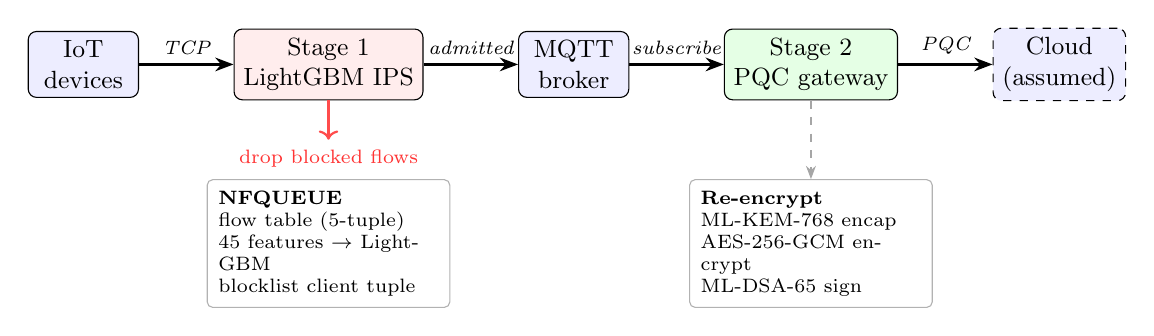
\begin{tikzpicture}[
    node distance=0.5cm and 0.4cm,
    box/.style={draw, rounded corners=3pt, fill=blue!7, minimum height=0.6cm, minimum width=1.4cm, font=\small, align=center},
    fwbox/.style={draw, rounded corners=3pt, fill=red!7, minimum height=0.6cm, font=\small, align=center},
    gwbox/.style={draw, rounded corners=3pt, fill=green!10, minimum height=0.6cm, font=\small, align=center},
    innerbox/.style={draw=gray!60, rounded corners=2pt, fill=white, font=\scriptsize, align=left, text width=2.8cm, inner sep=4pt},
    arr/.style={-Stealth, thick},
    darr/.style={-Stealth, dashed, gray!70},
    lbl/.style={font=\scriptsize\itshape, midway, above}
]
\node[box] (iot) {IoT\\devices};
\node[fwbox, right=1.2cm of iot, minimum width=2.0cm] (fw) {Stage 1\\LightGBM IPS};
\node[box, right=1.2cm of fw] (broker) {MQTT\\broker};
\node[gwbox, right=1.2cm of broker, minimum width=2.0cm] (gw) {Stage 2\\PQC gateway};
\node[box, right=1.2cm of gw, dashed] (cloud) {Cloud\\(assumed)};
\draw[arr] (iot) -- node[lbl]{TCP} (fw);
\draw[arr] (fw) -- node[lbl]{admitted} (broker);
\draw[arr] (broker) -- node[lbl]{subscribe} (gw);
\draw[arr] (gw) -- node[lbl]{PQC} (cloud);
\draw[->, red!70, thick] (fw.south) -- ++(0,-0.5) node[below, font=\scriptsize, red!80]{drop blocked flows};
\node[innerbox, below=1.0cm of fw] (fwd) {\textbf{NFQUEUE}\\flow table (5-tuple)\\45 features $\to$ LightGBM\\blocklist client tuple};
\node[innerbox, below=1.0cm of gw] (gwd) {\textbf{Re-encrypt}\\ML-KEM-768 encap\\AES-256-GCM encrypt\\ML-DSA-65 sign};
\draw[darr] (gw.south) -- (gwd.north);
\end{tikzpicture}
\caption{Two-stage gateway. Stage~1 classifies flows in the kernel packet path and blocks a client connection after an attack verdict; Stage~2 constructs a NIST Level~3 post-quantum envelope from messages it receives (dashed cloud: assumed, not evaluated).}
\label{fig:arch}
\end{figure*}

\subsection{Stage 1: LightGBM Flow Classifier and IPS}
\label{sec:stage1}

\textit{Interception:} An \texttt{iptables} rule sends packets for the broker port to NFQUEUE. A user-space callback parses IP/TCP (and UDP) headers with \texttt{dpkt}. To keep classification off the critical path, each packet is \emph{accepted back to the kernel before} the classifier runs; inference time therefore delays only later packets waiting in the queue, not the current one.

\textit{Flow State:} A bidirectional flow table keyed by the 5-tuple accumulates per-direction packet and byte counts, packet-length lists, inter-arrival times (IAT), TCP flag counts, and header lengths. A flow is classified 1)~when it terminates with FIN or RST after a configurable minimum number of packets (3 in the attack-only session and 20 in the combined session; shorter flows are never classified); 2)~every $N$ packets for long-lived connections such as publish floods ($N$ is configurable; logged flows reach at most 10 packets in the attack-only session and 50 in the combined session); and 3)~by a background reaper when idle for 10~s.

\textit{Features:} Each flow becomes the 45-dimensional CICIoMT2024 feature vector: duration and rate; per-direction SYN/ACK/PSH/FIN/RST/ECE/CWR counts; protocol indicators; packet-length total, minimum, maximum, mean, and standard deviation; mean IAT; derived Magnitude, Radius, Covariance, Variance, and Weight; and mean header length.

\textit{Classifier:} Features are standardized and passed to a 21-class LightGBM model~\cite{lightgbm2017} (benign plus 20 attack classes). A flow is labelled an attack when the arg-max class is not benign and the benign probability is below $1-\tau$, with $\tau = 0.5$.

\textit{Prevention:} In IPS mode, an attack verdict adds the client side of the flow (client IP, protocol, client port, broker port) to a blocklist; later packets matching it are dropped in the callback, and an \texttt{iptables} drop rule for the same tuple is inserted. Normalizing to the client side avoids blocking the broker's own replies from port 1883. Because the key includes the client port, a new connection from the same host is not covered by an earlier block. In IDS mode, verdicts are logged and nothing is dropped.

\textit{Enforcement Timing:} Three intervals separate a flow's first packet from its first dropped packet: 1)~\emph{collection time}, until the flow reaches a classification trigger (minimum packet count with FIN/RST, every $N$ packets, or 10~s of idleness); 2)~\emph{classification processing time}, for feature extraction, inference, and decision; and 3)~\emph{enforcement delay}, from the verdict to the next packet of the blocked tuple. Every packet before the verdict is admitted to the broker. Stage~1 therefore cuts off the remainder of long-lived attack connections, such as publish floods, but cannot stop connections that finish before a verdict: flows shorter than the minimum packet count are never classified, and a flow classified on FIN/RST has already ended, so its block affects only that tuple. Short connect floods and scans can thus complete before any blocking decision.

\subsection{Stage 2: Post-Quantum Re-Encryption}
\label{sec:stage2}

For every message received on a device topic, Stage~2 executes Algorithm~\ref{alg:reenc}. If the device used an encrypted scheme, the gateway first recovers the plaintext with the device key. It then encapsulates a fresh ML-KEM-768 shared secret to the cloud public key, encrypts the plaintext with AES-256-GCM under that secret and a random 96-bit nonce, and signs the encoded envelope with the gateway's ML-DSA-65 key.

\begin{algorithm}[!t]
\caption{Stage 2 Re-Encryption of an Admitted Message $m$}
\label{alg:reenc}
\begin{algorithmic}[1]
\State $p \gets \textsc{DeviceDecrypt}(m)$ \Comment{identity if plaintext}
\State $(c_\mathrm{kem}, ss) \gets \textsc{ML-KEM-768.Encaps}(pk_\mathrm{cloud})$
\State $\eta \xleftarrow{\$} \{0,1\}^{96}$
\State $c_\mathrm{aes} \gets \textsc{AES-256-GCM}_{ss}(p, \eta)$
\State $M \gets \textsc{Encode}(id, seq, c_\mathrm{kem}, \eta, c_\mathrm{aes})$
\State $\sigma \gets \textsc{ML-DSA-65.Sign}(sk_\mathrm{gw}, M)$
\State \textbf{return} $\{id, seq, c_\mathrm{kem}, \eta, c_\mathrm{aes}, \sigma\}$ \Comment{envelope for the cloud}
\end{algorithmic}
\end{algorithm}

\textit{Signed Encoding:} $\textsc{Encode}$ outputs a fixed domain tag followed by the five fields $id$ (UTF-8), $seq$ (unsigned 64-bit, big-endian), $c_\mathrm{kem}$, $\eta$, and $c_\mathrm{aes}$, each prefixed by its 4-byte big-endian length. Length prefixes make the encoding unambiguous: two different field tuples can never produce the same signed bytes. The Stage~2 timings in Section~\ref{sec:res-pqc} were recorded with an earlier revision that signed the plaintext $p$; the two revisions differ only in the input to ML-DSA-65, which hashes its message before signing, so the envelope adds about 1.1~KB of hashing input per message. We expect this to change signing time by microseconds but have not re-measured it.

\textit{Security Properties:} By construction, a fresh encapsulation per message gives each message an independent key, so compromise of one message key does not expose others, and the IND-CCA2 security of ML-KEM-768 protects the uplink against A2 at NIST Level~3. ML-DSA-65 (EUF-CMA) over the encoded envelope gives integrity and gateway origin authentication against A3, and binding the signature to $(id, seq)$ allows a cloud receiver that tracks the last accepted $seq$ per device to reject replays. Signing the ciphertext rather than the plaintext also prevents an observer from confirming guesses of low-entropy sensor readings against a public signature. Cloud-side signature verification, decryption, and replay rejection are expected protocol properties, not experimentally demonstrated results (Section~\ref{sec:keys}). The device-to-gateway link keeps whatever scheme the device already uses (AES-256 under Grover retains 128-bit security), which meets G4 but does not add forward secrecy on that segment.

\subsection{Key Provisioning and Experimental Assumptions}
\label{sec:keys}

\textit{Provisioning:} Before the experiments, a single 256-bit master secret, written as 64 hexadecimal characters, is placed out of band in a local environment file on the experimental nodes. Each process loads it at start-up; it is never sent over MQTT or any other network channel.

\textit{Derivation:} Every key is derived from the master secret with HKDF-SHA256~\cite{rfc5869} (no salt) under a domain-separated context string that names the algorithm and, where applicable, the device, e.g., \texttt{aes:}$\langle id\rangle$, \texttt{ecdsa-p256:}$\langle id\rangle$, \texttt{kem:}$\langle alg\rangle$\texttt{:keypair}, and \texttt{sig:}$\langle alg\rangle$\texttt{:}$\langle id\rangle$\texttt{:keypair}. AES-256 and ChaCha20-Poly1305 keys are taken directly from HKDF output, and P-256 private keys are HKDF output reduced modulo the group order. PQC key pairs are produced by the standard liboqs key-generation routines while the liboqs random-number source is temporarily replaced, through its custom-RNG interface (\texttt{OQS\_randombytes\_custom\_algorithm}), by a callback that returns a 64-byte HKDF output repeated cyclically; after key generation, including on error, the system RNG is restored (\texttt{OQS\_randombytes\_switch\_algorithm}). The hook requires the bindings to use the same liboqs shared library; all real-liboqs PQC messages in the scheme comparison were accepted, which requires matching key pairs on client and gateway. Every node therefore reproduces the same key pairs without a key exchange. KEM key pairs are scoped per algorithm, so all devices encrypt to one gateway KEM key per algorithm; signature key pairs are scoped per device. Encapsulation randomness and AES-GCM nonces come from the system RNG.

\textit{Purpose and Measurement:} This setup makes runs reproducible and keeps key distribution out of the measured path: provisioning happens before any measurement and is not part of any reported latency. The scheme-comparison gateway is stateless and rederives the gateway KEM key pair and the sending device's verification key for every message. This regeneration falls inside the total handler time but outside the decapsulation, decryption, and verification timers, and Section~\ref{sec:res-matrix} reports the resulting non-cryptographic time separately. Stage~2 likewise derives its keys inside the handler, before its encapsulation timer starts.

\textit{Cloud Receiver:} The cloud receiver is an assumed deployment component; it is not implemented or evaluated. Stage~2 constructs the protected envelope at the gateway, and we measure gateway-side encapsulation, encryption, and signing; in the prototype the envelope is not transmitted, so delivery, decapsulation, decryption, signature verification, and replay rejection at a cloud receiver are not evaluated. As a stand-in for the cloud public key, Stage~2 encapsulates to the ML-KEM-768 key pair derived from the master secret and signs with an ML-DSA-65 key derived for a fixed relay identity. In a deployment, the cloud receiver would generate and hold its own ML-KEM private key, and the gateway would use an authenticated copy of the corresponding public key together with its own signing key.

\textit{Trust Assumptions:} The experiments assume a single trusted administrative domain. In the live sessions, clients, broker, gateway, and attack generators run on one Raspberry Pi~4B over loopback, and all nodes are controlled by the researchers. The master secret is assumed to be unavailable to attackers; the attack generators do not use it or any derived key. The secret is not rotated during the reported experiments. These are experimental assumptions, not security guarantees.

\textit{Limits of a Shared Secret:} A shared master secret is a single point of failure: whoever obtains it can derive every key derived from it, including device keys, the gateway's KEM private key, and the stand-in cloud key. Deterministic shared-seed key generation is a controlled-testbed convenience, not a recommended production provisioning method. A production deployment requires independently provisioned device keys, private keys protected in hardware (e.g., a secure element or TPM), separate cloud key management in which the gateway never holds the cloud private key, and key rotation and revocation. The reported encapsulation, decapsulation, signing, and verification times measure operations on keys already in memory and do not depend on how those keys were generated. Production key management (enrolment, certificate validation, hardware key access, rotation, and revocation) would add overhead that we do not measure.

\subsection{Implementation}

Both stages run on a Raspberry Pi~4B (BCM2711, four Cortex-A72 cores at 1.8~GHz, 4~GB LPDDR4) under Python~3.11. Stage~1 uses \texttt{NetfilterQueue}, \texttt{dpkt}, and LightGBM; Stage~2 uses \texttt{liboqs-python}~\cite{oqs2023}, the \texttt{cryptography} package for AES-GCM, and Paho-MQTT with Mosquitto. Timestamps come from \texttt{time.perf\_counter\_ns()}, and records are written by a background thread to avoid perturbing measurements.

% ═════════════════════════════════════════════════════════════════════════════
\section{Evaluation Methodology}
\label{sec:method}

\subsection{Offline Model Evaluation}

The LightGBM model was trained on 1,129,927 CICIoMT2024 flows and tested on 484,255 held-out flows with the same 45 features (multiclass objective, learning rate 0.05, 31 leaves; training time 17.6~s). We report per-class precision, recall, F1, accuracy, and macro-F1.

\subsection{Live Workloads}

\textit{Benign Clients:} Three generators model legitimate devices: a \emph{steady} sensor with a fixed publish interval, a \emph{burst} device that sends 5--20 messages at 10~msg/s and then idles for 3--15~s, and a \emph{mixed} device combining both. Each embeds a device identifier and a monotonic sequence number in every message.

\textit{Attack Clients:} Generators reproduce the CICIoMT2024 MQTT and TCP/IP attack families: MQTT connect flood, MQTT publish flood, TCP SYN flood, UDP flood, ICMP flood, port scan, malformed MQTT packets, slow-connection (Slowloris-style) exhaustion, and replay. An orchestrator runs each attack for a fixed window, optionally with benign clients running throughout.

\subsection{Live Sessions and Metrics}
\label{sec:protocol}

All live components (clients, attack generators, firewall, broker, and gateway) ran on the same Raspberry Pi and exchanged traffic over the loopback interface, so the measurements reflect gateway processing cost without network variance. We analyse two sessions.
\begin{itemize}
  \item \textit{Attack-Only Session (11~min):} Ten attack types were injected with no benign clients. It measures Stage~1 latency and prediction behaviour.
  \item \textit{Combined Session (20~min):} Three benign publishers (steady, mixed, burst), each restarted once during the session (six device identifiers in total), a monitoring subscriber, and the attack generators ran together, with both stages active and prevention enabled.
\end{itemize}
For both sessions we report Stage~1 verdicts, model confidence, and timing. Stage~2 per-message cost is reported for the combined session, for those messages that reached the gateway subscriber. Simultaneous operation of the two stages is measured; reliable end-to-end delivery, cloud reception, and full attack suppression are not.

\textit{Attribution Without Labels:} The generators did not record their flows, so no session carries per-flow ground truth, and model predictions are not treated as labels. For the combined session we attribute connections from the packet log instead. Because all processes share one host clock, each message received by Stage~2 is matched to the client-to-broker packet that carried it, identifying benign publisher connections; subscriber connections are identified by traffic direction, as they receive far more data from the broker than they send. Connections matching neither rule remain unattributed.

\subsection{PQC Measurements}

\textit{Stage~2 on Live Traffic:} We time KEM encapsulation, AES-GCM encryption, signing, their sum, and the full handler (MQTT callback to completion) for every message received by the gateway subscriber. These timers are gateway-side processing costs; they are not added to Stage~1 classification time to form an end-to-end latency, and they do not include broker transit or cloud delivery. The live benign clients publish unencrypted JSON, so $\textsc{DeviceDecrypt}$ is the identity and these messages carry no device-side PQC; Stage~2 alone applies post-quantum protection, at the gateway. The constructed envelope is logged and not forwarded.

\textit{Scheme Comparison:} This separate benchmark evaluates device-to-gateway PQC: clients encrypt padded payloads of 5,120, 10,240, and 102,400 bytes under ten configurations (Table~\ref{tab:matrix}), 600 messages per configuration and size (18,000 messages, all accepted), and the gateway times decapsulation, decryption, and verification. Security level $L$ is the minimum NIST level of the KEM and signature. The configurations were measured sequentially in one session each, without interleaving or repeated sessions. PQC operations use liboqs; P-256 ECDH and ECDSA use OpenSSL through Python's \texttt{cryptography} package. AES-256-GCM and ChaCha20-Poly1305 are symmetric-only reference configurations: they perform no public-key establishment or signature verification and are not security-equivalent alternatives to the asymmetric configurations.

\textit{Timer Boundaries:} The crypto timer is the sum of the key-establishment, decryption, and verification timers; Base64 decoding, JSON handling, and logging fall outside it but inside the total handler time. The timers are not perfectly equivalent across libraries: the ECDH timer includes parsing the ephemeral public point and the HKDF derivation of the AES key, whereas the PQC decapsulation timer covers liboqs decapsulation without equivalent Base64 parsing or a KDF. The ECDH+ECDSA handler caches its static ECDH key and the device verification keys, whereas the PQC handler regenerates its key pairs for every message outside the crypto timer.

% ═════════════════════════════════════════════════════════════════════════════
\section{Results}
\label{sec:results}

\subsection{Offline Classifier Performance}
\label{sec:res-offline}

On the held-out set the model reaches 97.85\% accuracy, 0.900 macro-F1, and 0.979 weighted F1 (Fig.~\ref{fig:offline}). Benign traffic is recognized with 0.979 precision and 0.979 recall, so about 2.1\% of benign test flows are assigned to an attack class. Volumetric TCP/IP attacks (SYN, TCP, UDP, ICMP DoS) and MQTT connect/publish floods reach F1 between 0.94 and 1.00. Performance drops for low-volume reconnaissance and protocol-abuse classes: ARP spoofing (0.834), OS scan (0.813), malformed MQTT (0.769), vulnerability scan (0.648), and ping sweep (0.127, only 56 test flows). These classes differ from benign traffic in a few packets rather than in rate, which flow statistics capture poorly.

\begin{figure}[!t]
\centering
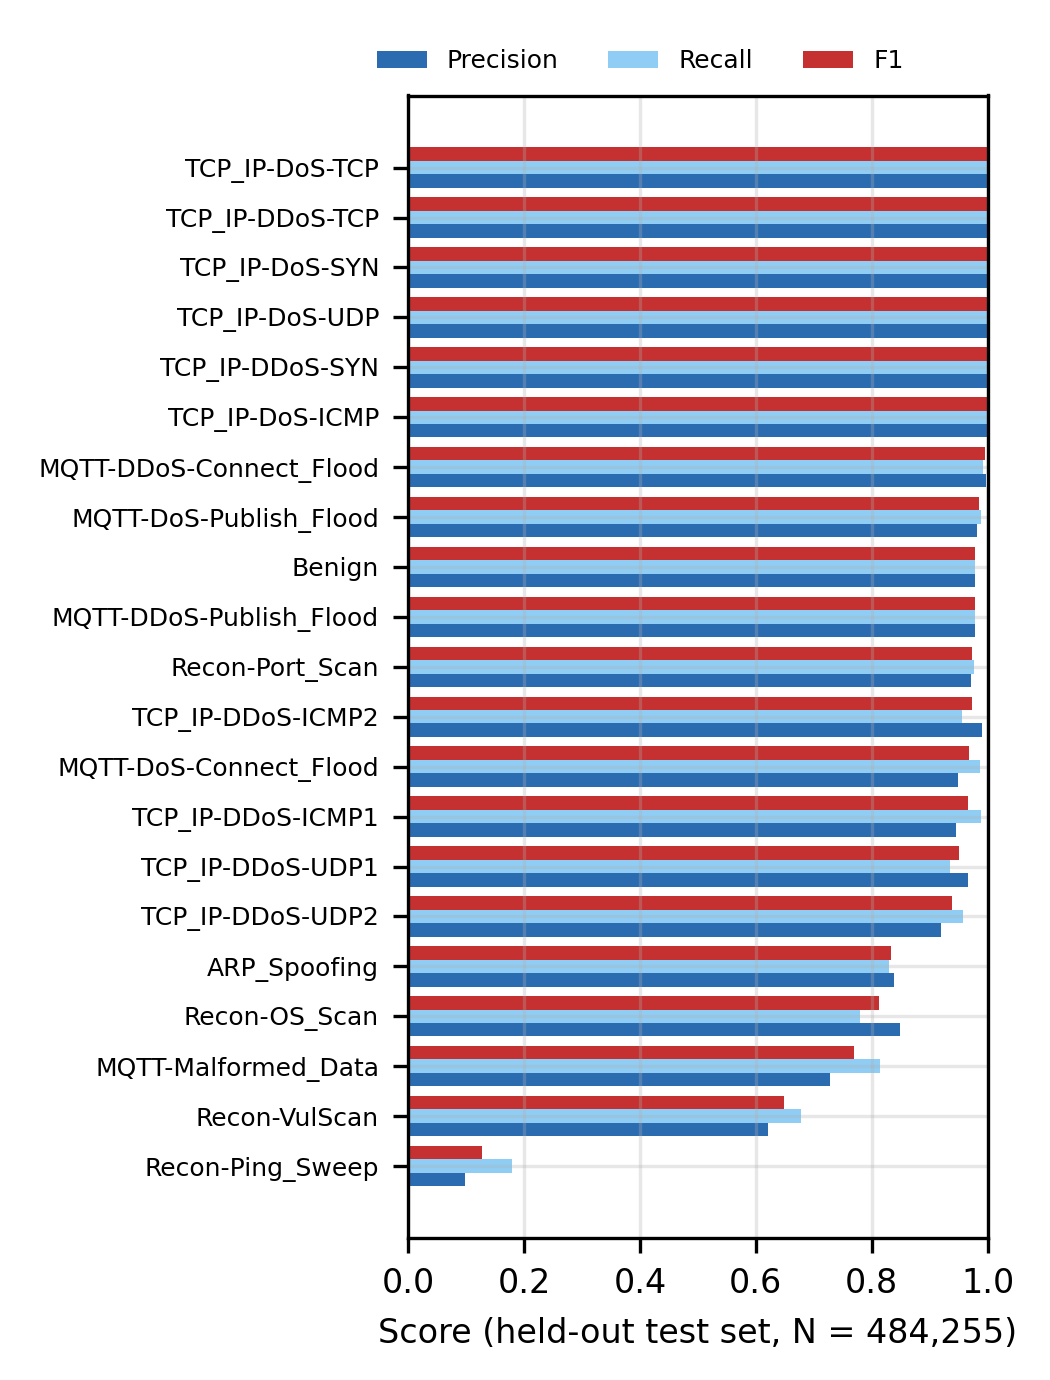
\includegraphics[width=\columnwidth]{fig_offline_per_class.png}
\caption{Per-class precision, recall, and F1 of the 21-class LightGBM model on the CICIoMT2024 held-out test set.}
\label{fig:offline}
\end{figure}

Variance, rate, and total size together account for 56.7\% of split gain, followed by protocol type (9.4\%) and duration (6.6\%) (Fig.~\ref{fig:fi}). The model therefore relies mainly on volume and timing, which explains both its strength on floods and its weakness on low-rate probes.

\begin{figure}[!t]
\centering
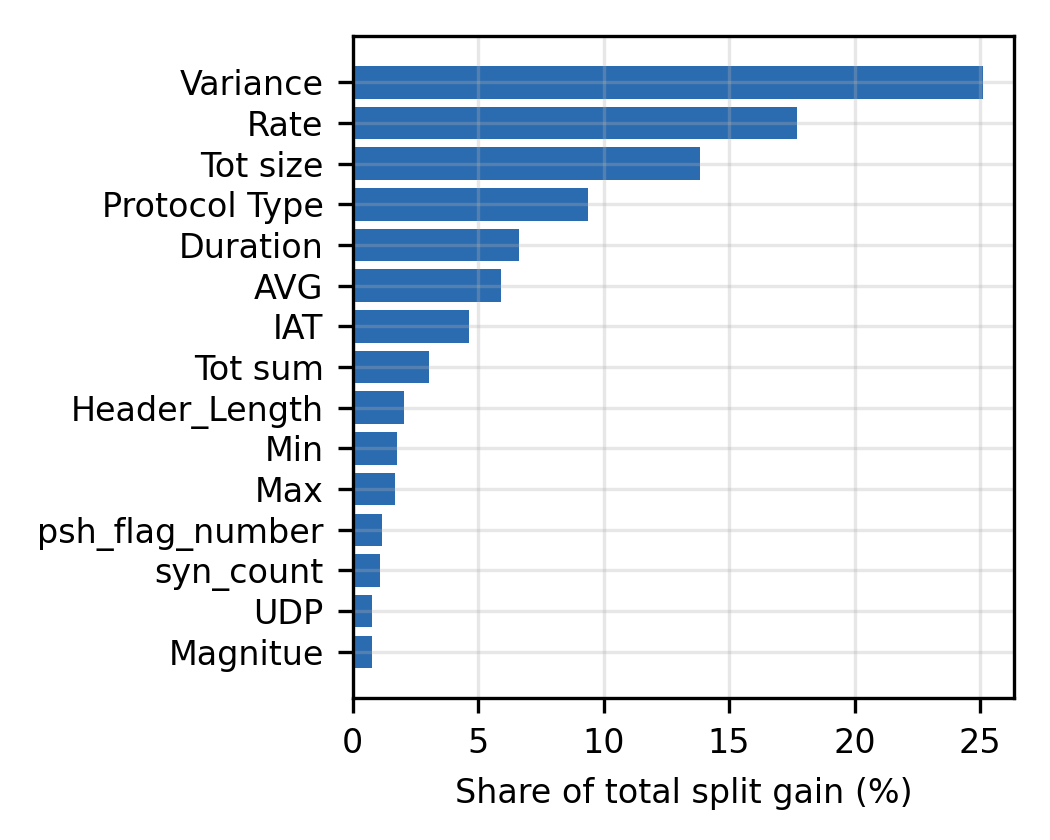
\includegraphics[width=\columnwidth]{fig_feature_importance.png}
\caption{Top-15 features by share of total LightGBM split gain.}
\label{fig:fi}
\end{figure}

\subsection{Stage 1 Live Performance}
\label{sec:res-ids}

\textit{Latency:} Table~\ref{tab:ids-latency} reports Stage~1 timing on the Pi over the 893 flows classified in the attack-only session (4,531 intercepted packets). LightGBM inference takes 0.435~ms on average, feature extraction plus inference plus decision 0.944~ms, and arrival of the triggering packet to verdict 1.201~ms for flows classified inline. Connect-flood flows, which are short and regular, are the fastest (0.871~ms); the other classes take 0.96--1.96~ms (e.g., OS scan 1.439~ms). These values are classification processing latency, not the time to detect and suppress an attack: before the trigger, flows spent 5.55~s on average (0.0004--95.9~s) collecting packets, all of which were admitted, and the time to the first enforced drop was not logged (Section~\ref{sec:stage1}). The processing cost is far below MQTT session setup times, so classification does not limit connection throughput at these rates.

\begin{table}[!t]
\centering
\caption{Stage~1 Live Timing on Raspberry Pi~4B by Predicted Class (Mean, ms). Inspect = Arrival of the Triggering Packet to Verdict, Inline-Triggered Flows Only; Excludes Packet Collection Time}
\label{tab:ids-latency}
\footnotesize
\setlength{\tabcolsep}{3pt}
\resizebox{\columnwidth}{!}{%
\begin{tabular}{lrrrr}
\toprule
\textbf{Predicted class} & \textbf{Flows} & \textbf{Infer.} & \textbf{Classify} & \textbf{Inspect} \\
\midrule
MQTT-DoS-Connect\_Flood  & 796 & 0.396 & 0.871 & 1.151 \\
Recon-OS\_Scan           & 28  & 0.762 & 1.439 & 1.571 \\
MQTT-DDoS-Connect\_Flood & 16  & 0.968 & 1.958 & 2.521 \\
MQTT-DDoS-Publish\_Flood & 13  & 0.699 & 1.467 & 1.850 \\
TCP\_IP-DDoS-SYN         & 13  & 0.689 & 1.491 & 1.713 \\
TCP\_IP-DDoS-UDP1        & 12  & 0.461 & 1.161 & 1.164 \\
MQTT-DoS-Publish\_Flood  & 8   & 0.474 & 1.189 & 1.379 \\
TCP\_IP-DDoS-TCP         & 4   & 0.438 & 0.963 & 1.286 \\
Other (ARP, port scan)   & 3   & --    & --    & --    \\
\midrule
\textbf{All}             & \textbf{893} & \textbf{0.435} & \textbf{0.944} & \textbf{1.201} \\
\bottomrule
\end{tabular}}
\end{table}

\textit{Prediction Behaviour:} All 893 classified flows of the attack-only session were predicted as attacks. Mean attack confidence was 0.997 (minimum 0.620), and 880 flows (98.5\%) exceeded 0.90. Flows had 3--10 packets (mean 4.6), so most verdicts were issued within the first few packets of a connection. Because flows were not tagged by generator, this share is a prediction rate, not a verified detection rate, and the predicted-class mix (89.1\% connect floods) is not a per-class accuracy; a labelled evaluation follows in Section~\ref{sec:res-labelled}.

\subsection{Stage 2 Re-Encryption Cost}
\label{sec:res-pqc}

Table~\ref{tab:stage2} and Fig.~\ref{fig:stage2} report Stage~2 cost for the 144 messages received by the gateway subscriber (188--213~B JSON payloads) in the combined session. The median re-encryption takes 0.156~ms: ML-DSA-65 signing dominates (0.094~ms), followed by ML-KEM-768 encapsulation (0.044~ms) and AES-GCM (0.009~ms). The mean of AES-GCM exceeds its P95 because two messages were delayed by scheduler preemption (maximum 1.609~ms). The full handler, including MQTT dispatch and JSON processing, has a median of 0.383~ms and P99 of 2.709~ms. Against a publish interval of seconds, this gateway-side cryptographic cost meets G5 by three orders of magnitude; G5 is not a measured end-to-end latency.

\begin{table}[!t]
\centering
\caption{Stage~2 Per-Message Gateway-Side Cost on Live Traffic (ms, $N = 144$ Messages Received by Stage~2, Real liboqs)}
\label{tab:stage2}
\footnotesize
\setlength{\tabcolsep}{3pt}
\resizebox{\columnwidth}{!}{%
\begin{tabular}{lrrrrr}
\toprule
\textbf{Operation} & \textbf{Median} & \textbf{Mean} & \textbf{P95} & \textbf{P99} & \textbf{Max} \\
\midrule
ML-KEM-768 encap.     & 0.044 & 0.047 & 0.065 & 0.103 & 0.215 \\
AES-256-GCM encrypt   & 0.009 & 0.030 & 0.024 & 0.398 & 1.609 \\
ML-DSA-65 sign        & 0.094 & 0.113 & 0.221 & 0.263 & 0.286 \\
\midrule
Re-encryption total   & 0.156 & 0.189 & 0.297 & 0.730 & 1.979 \\
Full gateway handler  & 0.383 & 0.488 & 0.613 & 2.709 & 11.477 \\
\bottomrule
\end{tabular}}
\end{table}

\begin{figure}[!t]
\centering
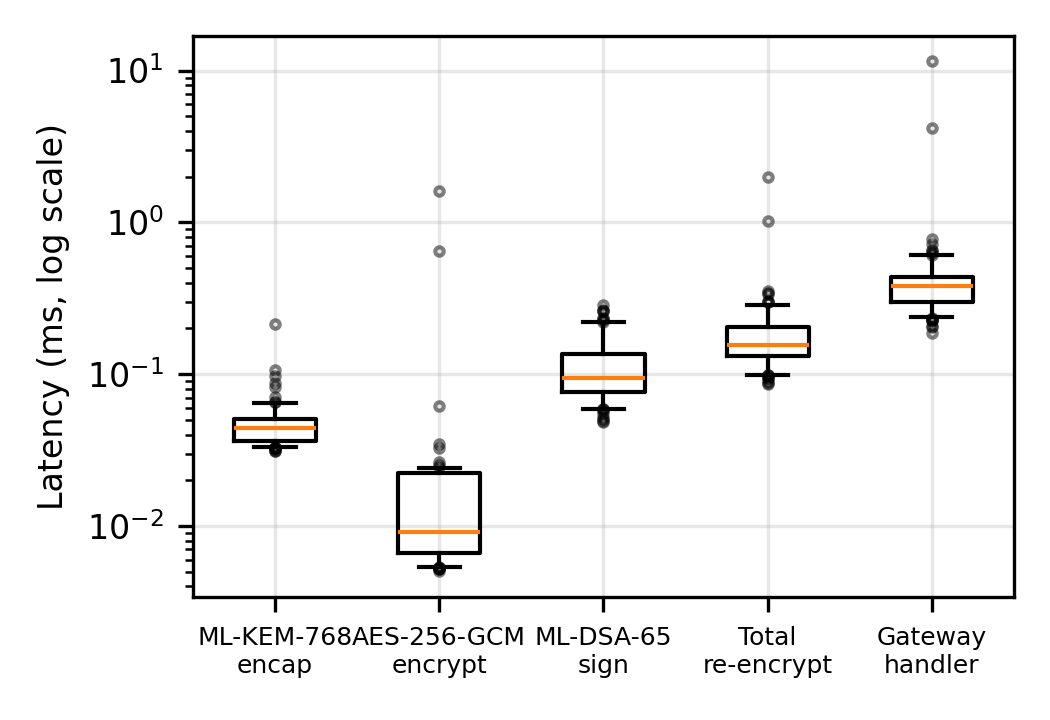
\includegraphics[width=\columnwidth]{fig_stage2_latency.png}
\caption{Distribution of Stage~2 per-message latency (box: interquartile range; whiskers: 5th--95th percentile).}
\label{fig:stage2}
\end{figure}

\textit{Bandwidth:} Re-encryption adds a fixed 4,425~B per message before encoding: the ML-KEM-768 ciphertext (1,088~B), the ML-DSA-65 signature (3,309~B), the nonce (12~B), and the GCM tag (16~B). This cost falls on the gateway-to-cloud uplink, not on the constrained device link.

\textit{Receiver Cost (Estimate):} A cloud receiver would perform the inverse operations: ML-KEM-768 decapsulation, AES-GCM decryption, and ML-DSA-65 verification. We do not measure a cloud receiver. As a reference, the gateway performs the same three operations in the separate scheme-comparison benchmark at a median of 0.772~ms per 5~KB message on the Raspberry Pi (Table~\ref{tab:matrix}), whereas live Stage~2 envelopes carried plaintext payloads of only about 200~B. This is a reference measurement, not a direct estimate of cloud latency; actual receiver cost depends on the cloud platform, software stack, and load, and excludes network transit.

\subsection{Choice of Post-Quantum Scheme}
\label{sec:res-matrix}

Table~\ref{tab:matrix} and Fig.~\ref{fig:matrix} compare ten configurations on the same gateway. Three tiers appear. In cryptographic time, ML-KEM pairings with ML-DSA or Falcon need 0.56--0.77~ms at 5~KB, about 36--53\% less than ECDH+ECDSA (1.21~ms), mainly because the measured ML-KEM decapsulation (0.13--0.19~ms) is 3--5$\times$ shorter than the P-256 ECDH timer (0.62~ms), whose boundary also includes point parsing and HKDF. The advantage depends on payload size: at 100~KB these pairings need 3.14--3.50~ms against 3.73~ms for ECDH+ECDSA. It also does not hold for total handler time (Table~\ref{tab:matrix}, Handler), where ECDH+ECDSA was faster (1.59~ms vs 1.85--2.32~ms at 5~KB) because its key objects were cached while the PQC key pairs were regenerated per message. SLH-DSA verification adds about 1~ms. FrodoKEM-640 (17.6~ms) and BIKE-L1 (36.1~ms) decapsulation dominate their pairings and produce the heaviest tails (P95 44--55~ms). At 100~KB, symmetric decryption grows to about 1.9~ms and narrows the gap: ML-KEM-768 + ML-DSA-65 costs 1.9$\times$ AES-only.

\begin{table*}[!t]
\centering
\caption{Gateway Receive Cost per Message (Median, ms) and Serialized MQTT Message Size. $L$ = Minimum NIST Level; $N = 600$ per Cell; Crypto = Decapsulation + Decryption + Verification Where Applicable; Handler = Total Gateway Handler Time, Including Per-Message PQC Key Regeneration (Classical Keys Cached)}
\label{tab:matrix}
\footnotesize
\begin{tabular}{lcrrrrrrrr}
\toprule
 & & \multicolumn{6}{c}{\textbf{5 KB payload}} & \multicolumn{2}{c}{\textbf{100 KB}} \\
\cmidrule(lr){3-8}\cmidrule(lr){9-10}
\textbf{Scheme (KEM + signature)} & \textbf{L} & \textbf{Decap} & \textbf{Verify} & \textbf{Crypto} & \textbf{P95} & \textbf{Handler} & \textbf{Msg. (B)} & \textbf{Crypto} & \textbf{Handler} \\
\midrule
ChaCha20-Poly1305          & -- & --     & --    & 0.073  & 0.143  & 0.403   & 7,327  & 0.424  & 2.371 \\
AES-256-GCM                & -- & --     & --    & 0.143  & 0.337  & 0.474   & 7,314  & 1.861  & 3.829 \\
ECDH + ECDSA P-256         & -- & 0.621  & 0.453 & 1.206  & 2.911  & 1.587   & 7,577  & 3.725  & 5.629 \\
\midrule
ML-KEM-512 + ML-DSA-44     & 1  & 0.130  & 0.260 & 0.562  & 1.514  & 1.852   & 11,604 & 3.283  & 6.177 \\
ML-KEM-512 + Falcon-512    & 1  & 0.129  & 0.279 & 0.572  & 1.456  & 22.472  & 9,253  & 3.140  & 25.954 \\
ML-KEM-768 + ML-DSA-65     & 3  & 0.194  & 0.433 & 0.772  & 2.125  & 2.321   & 13,216 & 3.497  & 6.603 \\
ML-KEM-768 + SLH-DSA-128s  & 1  & 0.167  & 1.363 & 1.723  & 2.317  & 156.515 & 19,293 & 4.458  & 161.630 \\
FrodoKEM-640 + ML-DSA-65   & 1  & 17.600 & 0.345 & 18.107 & 44.248 & 36.927  & 24,774 & 20.398 & 40.659 \\
FrodoKEM-640 + SLH-DSA-128s& 1  & 17.859 & 1.374 & 19.410 & 43.616 & 193.054 & 30,851 & 21.858 & 196.846 \\
BIKE-L1 + ML-DSA-44        & 1  & 36.126 & 0.248 & 36.550 & 54.794 & 81.711  & 12,677 & 39.093 & 85.673 \\
\bottomrule
\end{tabular}
\end{table*}

\begin{figure*}[!t]
\centering
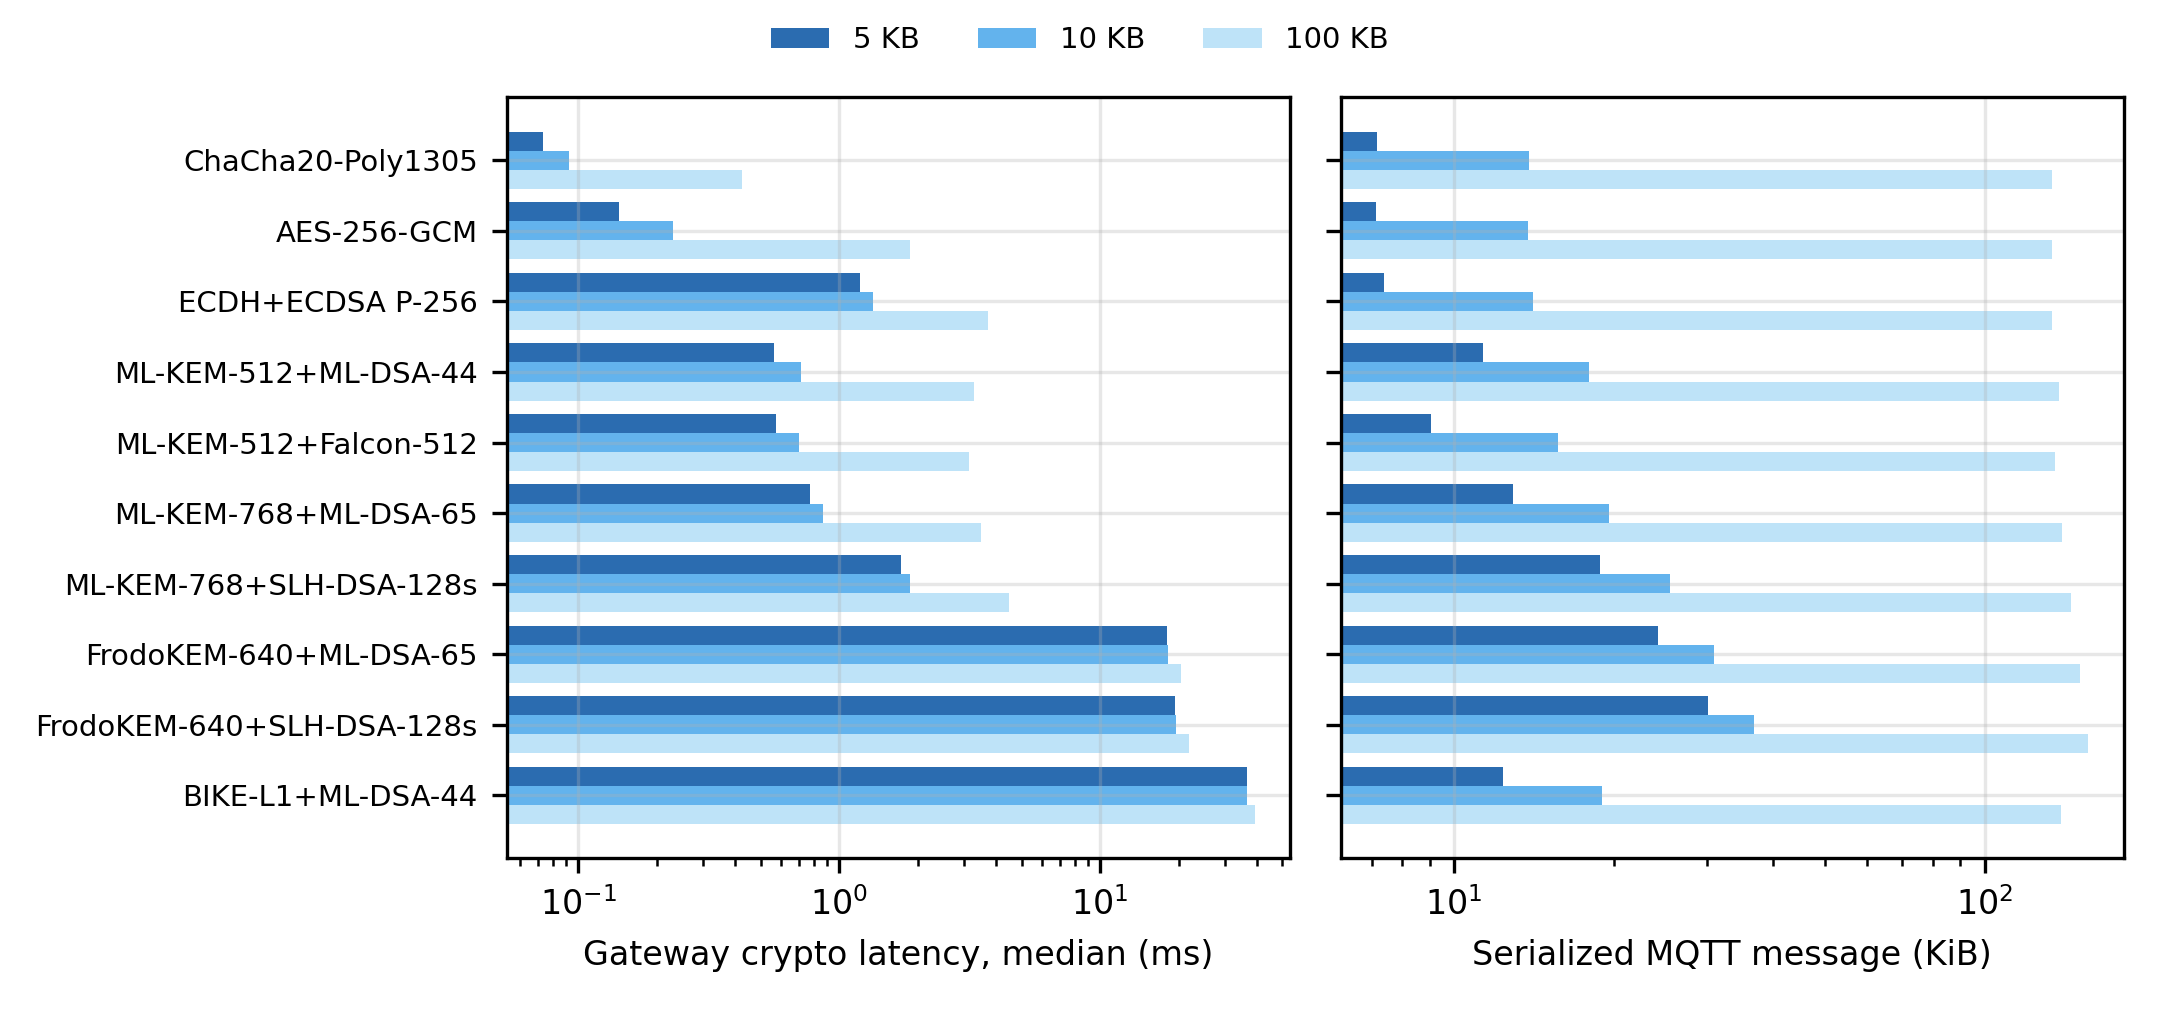
\includegraphics[width=0.9\textwidth]{fig_scheme_matrix.png}
\caption{Gateway cryptographic latency (left) and serialized message size (right) for ten configurations at three payload sizes (log scales).}
\label{fig:matrix}
\end{figure*}

\textit{Message Size:} Even AES-only expands a 5,120-byte payload to 7,314~B (+43\%) because of Base64 encoding and JSON metadata. Post-quantum material enlarges the 5~KB message by 1.27$\times$ (Falcon-512) to 4.22$\times$ (FrodoKEM + SLH-DSA) over AES-only, but only by 1.4--17\% at 100~KB, which favours batching small readings before protection.

\textit{Key Regeneration:} The PQC benchmark handler is stateless: it rederives the gateway KEM key pair and the device verification key for each message. The resulting non-cryptographic handler time, which includes key regeneration together with decoding, JSON handling, and logging, is 1.3--1.6~ms for ML-KEM/ML-DSA, 22~ms for Falcon-512, 19~ms for FrodoKEM, 45~ms for BIKE, and 155--174~ms for SLH-DSA, about 90$\times$ the cryptographic work. These figures are not pure key-generation latency: about 0.35~ms of non-cryptographic time is also observed in the AES-only, ChaCha20, and cached ECDH+ECDSA configurations. Practical gateways should cache keys per device and algorithm. Caching is expected to remove most of this overhead and to make Falcon and SLH-DSA viable, but a key-cached PQC handler was not measured.

\subsection{Both Stages Combined}
\label{sec:res-e2e}

In the combined session, Stage~1 intercepted 4,253 packets and issued 37 flow verdicts: 36 attack (16 MQTT-DDoS-Publish\_Flood, 9 MQTT-DoS-Publish\_Flood, 6 TCP\_IP-DDoS-UDP1, 3 TCP\_IP-DoS-TCP, 2 MQTT-DDoS-Connect\_Flood) and 1 benign. Mean inference time was 0.906~ms and mean classification time 2.075~ms, about twice the attack-only value, because flows were longer (up to 50 packets) and both stages shared the Pi. Stage~2 re-encrypted 144 benign messages that reached its MQTT callback, with the costs in Table~\ref{tab:stage2}. Those 144 records are gateway-side constructions of the protected envelope; they are not cloud deliveries, and they are not all of the benign messages that Stage~1 admitted to the broker. Benign clients did not log every sequence number they sent, so a delivery ratio cannot be computed from the existing files.

\textit{Blocked Connections:} Table~\ref{tab:blocked} attributes the 36 blocked connections using the method of Section~\ref{sec:protocol}. At least 11 were benign publishers and 9 were subscriber connections, including the gateway's own; the single benign verdict was a subscriber connection that was reclassified as an attack 15~s later. All six UDP flows to the broker port were attack traffic, as no benign client uses UDP. Because packets are accepted before classification, each blocked TCP connection delivered 13--33 client-to-broker packets before its verdict. A further 216 TCP connections, mostly of 10--14 packets, stayed below the 20-packet minimum and were never classified, so they reached the broker unfiltered.

\begin{table}[!t]
\centering
\caption{Blocked Connections in the Combined Session by Inferred Role}
\label{tab:blocked}
\footnotesize
\setlength{\tabcolsep}{3pt}
\resizebox{\columnwidth}{!}{%
\begin{tabular}{lrl}
\toprule
\textbf{Inferred role} & \textbf{Blocked} & \textbf{Attribution basis} \\
\midrule
Benign publisher            & 11 & Carried a message received by Stage~2 \\
Subscriber (gateway, monitor) & 9  & Broker-to-client data dominates \\
Publisher, unattributed     & 7  & No message reached Stage~2 \\
Short TCP flows (21 pkts)   & 3  & Origin unknown \\
UDP to broker port          & 6  & No benign client uses UDP \\
\midrule
\textbf{Total}              & \textbf{36} & \\
\bottomrule
\end{tabular}}
\end{table}

\textit{Effect on Stage~2:} Gateway receipts of benign messages paused from 0.3 to 4.1~min and from 4.3 to 6.1~min after the session start, and stopped at 6.3~min, two seconds after the fourth subscriber-like connection was blocked, although the session ran for 20~min. Each pause begins at a subscriber block in the packet log, which is consistent with Stage~1 cutting off the gateway's MQTT input, but the association is temporal rather than labelled: the logs do not record whether a blocked tuple belonged to the gateway process, nor whether unpublished benign messages were dropped, delayed, or never sent. Simultaneous operation of the two stages is therefore demonstrated only while the gateway subscriber remains connected. The Stage~1 classifier treats long-lived infrastructure clients like any other flow: a gateway that hosts its own MQTT clients behind the IPS must exempt them from blocking.

\subsection{Labelled Live Detection}
\label{sec:res-labelled}

\TODO{Fill from the labelled re-run: each process bound to its own loopback address (gateway, monitor, benign publishers, attackers), ground-truth sidecar logs, benign send logs, drop counters, identical classification settings in all runs, three repetitions. Runs: R1 benign only (IDS mode); R2 each attack alone (IDS); R3 benign + attacks (IDS); R4 benign + attacks (IPS, infrastructure allow-listed); R5 same without allow-list.}

\begin{table}[!t]
\centering
\caption{Live Detection by Traffic Source in IDS Mode (Mean $\pm$ SD Over Three Runs)}
\label{tab:live-detect}
\footnotesize
\setlength{\tabcolsep}{3pt}
\begin{tabular}{lrrr}
\toprule
\textbf{Source} & \textbf{Flows} & \textbf{Flagged} & \textbf{TPR / FPR} \\
\midrule
\TODO{one row per attack family} & -- & -- & -- \\
Benign publishers & -- & -- & -- \\
\midrule
\multicolumn{4}{l}{Precision, recall, F1: \TODO{}} \\
\bottomrule
\end{tabular}
\end{table}

\begin{table}[!t]
\centering
\caption{Effect of Inline Blocking (IPS Mode, Mean $\pm$ SD Over Three Runs)}
\label{tab:ips-effect}
\footnotesize
\setlength{\tabcolsep}{3pt}
\begin{tabular}{lrr}
\toprule
\textbf{Metric} & \textbf{Allow-list} & \textbf{No allow-list} \\
\midrule
Benign delivery ratio                 & -- & -- \\
Attack packets before verdict         & -- & -- \\
Attack packets dropped                & -- & -- \\
Attack flows never classified         & -- & -- \\
Infrastructure connections blocked    & -- & -- \\
\bottomrule
\end{tabular}
\end{table}

% ═════════════════════════════════════════════════════════════════════════════
\section{Discussion}
\label{sec:discussion}

\subsection{Why the Two Stages Compose}

The stages address different adversaries at different layers, but simultaneous operation is not the same as experimentally validated end-to-end security or availability. Stage~1 acts in the packet path ahead of the broker, where long-lived floods can be cut off cheaply from flow statistics once classified, although packets before the verdict and short connections reach the broker. Stage~2 acts on messages that the gateway subscriber receives, constructing a post-quantum envelope; it does not, in this prototype, transmit that envelope, and it processes a message only while that subscriber remains connected. PQC work is therefore spent only on traffic that reaches Stage~2, not on packets that Stage~1 later drops, and long-term confidentiality of a transmitted envelope would not depend on the classifier being correct. The two stages also run as separate processes (packet callback vs.\ MQTT callback): Stage~1 inference can delay later packets waiting in the queue, but the Stage~1 and Stage~2 timers are not added to form an end-to-end latency.

\subsection{Deployment Guidance}

\begin{itemize}
  \item \textit{Scheme:} ML-KEM-768 + ML-DSA-65 gives NIST Level~3 for under 0.8~ms of gateway cryptographic time at 5~KB; its advantage over ECDH+ECDSA narrows with payload size, and PQC key caching would be needed for it to carry over to total handler time, which we have not measured; ML-KEM-512 + Falcon-512 is the most bandwidth-efficient Level~1 option; FrodoKEM and BIKE suit only latency-tolerant links.
  \item \textit{Keys:} Cache key pairs per device and algorithm; per-message derivation dominates cost for Falcon and SLH-DSA.
  \item \textit{Bandwidth:} The fixed PQC overhead is large for small messages; batch readings where latency allows.
  \item \textit{IPS Policy:} Exempt infrastructure clients (the gateway's own subscriber and monitoring clients) from blocking, start in IDS mode, calibrate the threshold on local benign traffic, and allow-list registered devices before enabling blocking.
\end{itemize}

\subsection{Limitations}
\label{sec:limits}

\begin{itemize}
  \item \textit{Testbed:} Clients, attackers, broker, and gateway ran on one Raspberry Pi over loopback, so network effects and multi-device contention are not captured.
  \item \textit{Ground Truth:} The live sessions analysed in Sections~\ref{sec:res-ids} and~\ref{sec:res-e2e} carry no per-flow labels, so they yield predictions and an inferred attribution of blocked connections, not TPR, FPR, or a confusion matrix. Each of these sessions was run once.
  \item \textit{Enforcement Timing:} The logs record classification processing time and packet collection time, but not dropped packets or the time from flow start to the first enforced drop, so attack suppression is not quantified.
  \item \textit{Signature Revision:} Stage~2 timings were recorded before the signature input was changed from the plaintext to the encoded envelope (Section~\ref{sec:stage2}) and have not been re-measured.
  \item \textit{Dataset Shift:} The model is trained on CICIoMT2024 and may not match other deployments; retraining or calibration on local traffic is needed.
  \item \textit{Evasion:} An adversary who knows the features can shape traffic to look benign; adversarial robustness is not evaluated.
  \item \textit{Scheme Benchmark:} Configurations ran sequentially without independent repetitions, timer boundaries are implementation-specific (Section~\ref{sec:method}), and the PQC and classical handlers use different key-caching policies.
  \item \textit{Runtime:} Python adds dispatch and parsing overhead that a C implementation would avoid; absolute latencies are therefore conservative.
  \item \textit{Joint Evaluation:} The combined session shows both stages running on one host, not continuous availability under attack and not cloud delivery. Stage~2 processed only the 144 messages that reached its subscriber; HNDL confidentiality and uplink authentication (G2, G3) are properties of the constructed envelope, not experimentally demonstrated against a cloud observer or active attacker.
  \item \textit{Cloud Receiver:} The cloud receiver is assumed, not implemented; its cost is only a reference from gateway receive-side measurements, and WAN latency is not included (Section~\ref{sec:keys}).
  \item \textit{Not Measured:} End-to-end message latency, benign-message delivery ratio, energy, WAN transit time, and multi-gateway scaling.
  \item \textit{Key Management:} All keys derive from one shared master secret under the trust assumptions of Section~\ref{sec:keys}; this is a testbed convenience and a single point of failure, not a production provisioning scheme.
\end{itemize}

% ═════════════════════════════════════════════════════════════════════════════
\section{Conclusion}
\label{sec:conclusion}

We presented a two-stage MQTT gateway that classifies live MQTT-bound flows with a LightGBM model in the kernel packet path, blocks client connections flagged as attacks, and constructs an ML-KEM-768 + AES-256-GCM + ML-DSA-65 envelope on messages that reach Stage~2, and measured it on a Raspberry Pi~4B. Stage~1 needs under 1~ms of processing per classification, and Stage~2 needs a median 0.156~ms of cryptographic work per received message; these are separate gateway costs, not a measured end-to-end latency. Blocking takes effect only after a flow has collected enough packets, so short attack connections can complete first, and in the combined session the IPS also interrupted Stage~2's own subscriber. Across ten configurations, ML-KEM pairings with ML-DSA or Falcon needed less cryptographic time than ECDH+ECDSA at 5~KB, an advantage that narrows at 100~KB and that the per-message PQC key regeneration outweighed in total handler time; key caching is therefore expected, though not yet measured, to decide both this comparison and whether Falcon and SLH-DSA are practical. Live logs also show that an inline IPS must exempt the gateway's own MQTT clients, whose blocking stalled delivery to Stage~2. Future work will add energy measurements, distributed multi-node deployments, adversarially robust detection, and a native implementation.

\bibliographystyle{IEEEtran}
\bibliography{bib/references_journal}

\end{document}
